%
% This document contains the chapter about microstrip components.
%

\chapter{Microstrip components}
%\addcontentsline{toc}{chapter}{Microstrip components}
\label{sec:MScomponents}

\section{Single microstrip line}
%\addcontentsline{toc}{section}{Single microstrip line}

\begin{figure}[ht]
\begin{center}
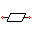
\includegraphics[width=12cm]{msline}
\end{center}
\caption{single microstrip line}
\label{fig:MSline}
\end{figure}
\FloatBarrier

The electrical parameters of microstrip lines which are required for
circuit design are impedance, attenuation, wavelength and propagation
constant.  These parameters are interrelated for all microstrips
assuming that the propagation mode is a transverse electromagnetic
mode, or it can be approximated by a transverse electromagnetic mode.

\subsection{Quasi-static characteristic impedance}
%\addcontentsline{toc}{subsection}{Quasi-static characteristic impedance}

\subsubsection{Wheeler}
%\addcontentsline{toc}{subsubsection}{Wheeler}

Harold A. Wheeler \cite{Wheeler2} formulated his synthesis and
analysis equations based upon a conformal mapping's approximation of
the dielectric boundary with parallel conductor strips separated by a
dielectric sheet.

\addvspace{12pt}

For wide strips ($W/h > 3.3$) he obtains the approximation
\begin{equation}
Z_{L}\left(W, h, \varepsilon_{r}\right) =
\frac{Z_{F0}}{2\sqrt{\varepsilon_{r}}}\cdot\frac{1}{\dfrac{W}{2h} + \dfrac{1}{\pi}\ln{4} + \dfrac{\varepsilon_{r} + 1}{2\pi \varepsilon_{r}} \ln{\left(\dfrac{\pi e}{2}\left(\dfrac{W}{2h} + 0.94\right)\right)} + \dfrac{\varepsilon_{r} - 1}{2\pi \varepsilon_{r}^{2}}\cdot \ln{\dfrac{e\pi^{2}}{16}}}
\end{equation}

For narrow strips ($W/h \le 3.3$) he obtains the approximation
\begin{equation}
Z_{L}\left(W, h, \varepsilon_{r}\right) =
\frac{Z_{F0}}{\pi \sqrt{2 \left(\varepsilon_{r} + 1\right)}} \cdot \left(\ln{\left(\frac{4h}{W} + \sqrt{\left(\frac{4h}{W}\right)^{2} + 2}\right)} - \frac{1}{2}\cdot \frac{\varepsilon_{r} - 1}{\varepsilon_{r} + 1}\left(\ln{\frac{\pi}{2}} + \frac{1}{\varepsilon_{r}} \ln{\frac{4}{\pi}}\right)\right)
\end{equation}

The formulae are applicable to alumina-type substrates ($8 \le
\varepsilon_r \le 12$) and have an estimated relative error less than
1 per cent.

\begin{figure}[ht]
\begin{center}
\psfrag{impedance ZL in Ohm}{$\mathrm{\text{impedance }Z_{L}\text{ in }[\ohm]}$}
\psfrag{normalised strip width W/h}{normalised strip width W/h}
\includegraphics[width=0.95\linewidth]{mszl}
\end{center}
\caption{characteristic impedance as approximated by Hammerstad for $\varepsilon_{r}$ = $1.0$ (air), $3.78$ (quartz) and $9.5$ (alumina)}
\label{fig:mszl}
\end{figure}
\FloatBarrier

\subsubsection{Schneider}
%\addcontentsline{toc}{subsubsection}{Schneider}

The following formulas obtained by rational function approximation
give accuracy of $\pm 0.25\%$ for $0 \le W/h \le 10$ which is the
range of importance for most engineering applications.  M.V. Schneider
\cite{Schneider} found these approximations for the complete elliptic
integrals of the first kind as accurate as $\pm 1\%$ for $W/h > 10$.

\begin{equation}
Z_L = \dfrac{Z_{F0}}{\sqrt{\varepsilon_{r_{eff}}}}\cdot
\begin{cases}
\begin{array}{ll}
\dfrac{1}{2\pi}\cdot \ln{\left(\dfrac{8\cdot h}{W} + \dfrac{W}{4\cdot h}\right)} & \textrm{ for } \dfrac{W}{h} \le 1\\
&\\
\dfrac{1}{\dfrac{W}{h} + 2.42 - 0.44\cdot\dfrac{h}{W} + \left(1 - \dfrac{h}{W}\right)^6} & \textrm{ for } \dfrac{W}{h} > 1\\
\end{array}
\end{cases}
\end{equation}

\subsubsection{Hammerstad and Jensen}
%\addcontentsline{toc}{subsubsection}{Hammerstad and Jensen}

The equations for the single microstrip line presented by
E. Hammerstad and {\O}. Jensen \cite{Hammerstad} are based upon an
equation for the impedance of microstrip in an homogeneous medium and
an equation for the microstrip effective dielectric constant.  The
obtained accuracy gives errors at least less than those caused by
physical tolerances and is better than $0.01\%$ for $W/h \le 1$ and
$0.03\%$ for $W/h \le 1000$.

\begin{align}
\label{eq:HandJZL0}
Z_{L1}\left(W, h\right) &=
\frac{Z_{F0}}{2\pi}\cdot\ln{\left(f_{u}\frac{h}{W} + \sqrt{1 + \left(\frac{2h}{W}\right)^{2}}\right)}\\
\label{eq:HandJZL0Er}
Z_{L}\left(W, h, \varepsilon_{r}\right) &= \dfrac{Z_{L1} \left(W, h\right)}{\sqrt{\varepsilon_{r}}} = \frac{Z_{F0}}{2\pi\cdot\sqrt{\varepsilon_{r}}}\cdot\ln{\left(f_{u}\frac{h}{W} + \sqrt{1 + \left(\frac{2h}{W}\right)^{2}}\right)}
\end{align}

with
\begin{align}
f_{u} &= 6 + \left(2\pi - 6\right)\cdot\exp{\left(-\left(30.666\cdot\frac{h}{W}\right)^{0.7528}\right)}
\end{align}

The comparison of the expression given for the quasi-static impedance
as shown in fig. \ref{fig:mscomparezl} has been done with respect to
E. Hammerstad and {\O}. Jensen.  It reveals the advantage of closed-form
expressions.  The impedance step for Wheelers formulae at $W/h = 3.3$
is approximately $0.1\ohm$.

\begin{figure}[ht]
\begin{center}
\psfrag{deviation of impedance ZL in \%}{$\mathrm{\text{deviation of impedance }Z_{L}\text{ in }[\%]}$}
\psfrag{normalised strip width W/h}{normalised strip width W/h}
\includegraphics[width=0.95\linewidth]{mscomparezl}
\end{center}
\caption{characteristic impedance in comparison for $\varepsilon_{r} = 9.8$}
\label{fig:mscomparezl}
\end{figure}
\FloatBarrier

\subsection{Quasi-static effective dielectric constant}
%\addcontentsline{toc}{subsection}{Quasi-static effective dielectric constant}

\subsubsection{Wheeler}
%\addcontentsline{toc}{subsubsection}{Wheeler}

Harold A. Wheeler \cite{Wheeler} gives the following approximation for
narrow strips ($W/h < 3$) based upon the characteristic impedance
$Z_L$.  The estimated relative error is less than 1\%.
\begin{equation}
\varepsilon_{r_{eff}} = \frac{\varepsilon_{r} + 1}{2} + \frac{Z_{F0}}{2\pi Z_{L}}\cdot \frac{\varepsilon_{r} - 1}{2}\cdot \left(\ln{\frac{\pi}{2}} + \frac{1}{\varepsilon_{r}} \ln{\frac{4}{\pi}}\right)
\end{equation}

For narrow strips ($W/h \le 1.3$):
\begin{equation}
\varepsilon_{r_{eff}} = \dfrac{1 + \varepsilon_r}{2}\cdot \left(\dfrac{A}{A - B}\right)^2
\end{equation}
with
\begin{align}
A &= \ln{\left(8\dfrac{h}{W}\right)} + \dfrac{1}{32}\cdot\left(\dfrac{W}{h}\right)^2\\
B &= \dfrac{1}{2}\cdot \dfrac{\varepsilon_r - 1}{\varepsilon_r + 1} \cdot\left(\ln{\dfrac{\pi}{2}} + \dfrac{1}{\varepsilon_r}\ln{\dfrac{4}{\pi}}\right)
\end{align}

For wide strips ($W/h > 1.3$):
\begin{equation}
\varepsilon_{r_{eff}} = \varepsilon_r\cdot\left(\dfrac{E - D}{E}\right)^2
\end{equation}
with
\begin{align}
D &= \dfrac{\varepsilon_r - 1}{2\pi \varepsilon_r}\cdot\left(\ln{\left(\dfrac{\pi e}{2}\left(\dfrac{W}{2h} + 0.94\right)\right)} - \dfrac{1}{\varepsilon_r} \ln{\dfrac{e\pi^{2}}{16}}\right)\\
E &= \dfrac{1}{2}\cdot\dfrac{W}{h} + \dfrac{1}{\pi}\cdot \ln{\left(\pi e \dfrac{W}{h} + 16.0547\right)}
\end{align}

\subsubsection{Schneider}
%\addcontentsline{toc}{subsubsection}{Schneider}

The approximate function found by M.V. Schneider \cite{Schneider} is
meant to have an accuracy of $\pm 2\%$ for $\varepsilon_{r_{eff}}$ and
an accuracy of $\pm 1\%$ for $\sqrt{\varepsilon_{r_{eff}}}$.

\begin{equation}
\varepsilon_{r_{eff}} = \dfrac{\varepsilon_{r} + 1}{2} + \dfrac{\varepsilon_{r} - 1}{2}\cdot\dfrac{1}{\sqrt{1 + 10\dfrac{h}{W}}}
\end{equation}

\subsubsection{Hammerstad and Jensen}
%\addcontentsline{toc}{subsubsection}{Hammerstad and Jensen}

The accuracy of the E. Hammerstad and {\O}. Jensen \cite{Hammerstad} model
is better than 0.2\% at least for $\varepsilon_r < 128$ and $0.01 \le
W/h \le 100$.
\begin{equation}
\label{eq:HandJErEff}
\varepsilon_{r_{eff}}\left(W, h, \varepsilon_r\right) = \frac{\varepsilon_{r} + 1}{2} + \frac{\varepsilon_{r} - 1}{2}\cdot\left(1 + 10\frac{h}{W}\right)^{-ab}
\end{equation}

with
\begin{align}
\label{eq:HandJa}
a\left(u\right) &= 1 + \frac{1}{49}\cdot\ln{\left(\frac{u^{4} + \left(u/52\right)^{2}}{u^{4} + 0.432}\right)} + \frac{1}{18.7}\cdot\ln{\left(1 + \left(\frac{u}{18.1}\right)^{3}\right)}\\
\label{eq:HandJb}
b\left(\varepsilon_r\right) &= 0.564\cdot\left(\frac{\varepsilon_{r} - 0.9}{\varepsilon_{r} + 3}\right)^{0.053}\\
u &= \frac{W}{h}
\end{align}

\subsection{Strip thickness correction}
%\addcontentsline{toc}{subsection}{Strip thickness correction}

The formulas given for the quasi-static characteristic impedance and
effective dielectric constant in the previous sections are based upon
an infinite thin microstrip line thickness $t = 0$.  A finite
thickness $t$ can be compensated by a reduction of width.  That means
a strip with the width $W$ and the finite thickness $t$ appears to be
a wider strip.

\subsubsection{Wheeler}
%\addcontentsline{toc}{subsubsection}{Wheeler}

Harold A. Wheeler \cite{Wheeler} proposes the following equation to
account for the strip thickness effect based on free space without
dielectric.
\begin{equation}
\Delta W_1 = \dfrac{t}{\pi} \ln{\dfrac{4 e}{\sqrt{\left(\dfrac{t}{h}\right)^2 + \left(\dfrac{1/\pi}{W/t + 1.10}\right)}}}
\end{equation}

For the mixed media case with dielectric he obtains the approximation
\begin{equation}
\Delta W_r = \dfrac{1}{2} \Delta W_1 \left(1 + \dfrac{1}{\varepsilon_r}\right)
\end{equation}

\subsubsection{Schneider}
%\addcontentsline{toc}{subsubsection}{Schneider}

M.V. Schneider \cite{Schneider} derived the following approximate
expressions.
\begin{equation}
\Delta W =
\begin{cases}
\begin{array}{ll}
\dfrac{t}{\pi}\cdot\left(1 + \ln{\dfrac{4\cdot\pi\cdot W}{t}}\right) & \textrm{ for } \dfrac{W}{h} \le \dfrac{1}{2\pi}\\
&\\
\dfrac{t}{\pi}\cdot\left(1 + \ln{\dfrac{2\cdot h}{t}}\right) & \textrm{ for } \dfrac{W}{h} > \dfrac{1}{2\pi}\\
\end{array}
\end{cases}
\end{equation}

Additional restrictions for applying these expressions are $t \ll h$,
$t < W/2$ and $t/\Delta W < 0.75$.  Notice also that the ratio $\Delta
W / t$ is divergent for $t \rightarrow 0$.

\subsubsection{Hammerstad and Jensen}
%\addcontentsline{toc}{subsubsection}{Hammerstad and Jensen}

E. Hammerstad and {\O}. Jensen are using the method described by Wheeler
\cite{Wheeler} to account for a non-zero strip thickness.  However,
some modifications in his equations have been made, which give better
accuracy for narrow strips and for substrates with low dielectric
constant.  For the homogeneous media the correction is
\begin{equation}
\Delta W_1 = \dfrac{t}{h\cdot\pi} \ln{\left(1 + \dfrac{4e}{\dfrac{t}{h}\cdot \coth^2{\sqrt{6.517 W}}}\right)}
\end{equation}

and for the mixed media the correction is
\begin{equation}
\Delta W_r = \dfrac{1}{2} \Delta W_1 \left(1 + \text{sech} \sqrt{\varepsilon_r - 1}\right)
\end{equation}

By defining corrected strip widths, $W_1 = W + \Delta W_1$ and $W_r =
W + \Delta W_r$, the effect of strip thickness may be included in the
equations \eqref{eq:HandJZL0} and \eqref{eq:HandJErEff}.
\begin{align}
Z_L \left(W, h, t, \varepsilon_r\right) &= \dfrac{Z_{L1} \left(W_r, h\right)}{\sqrt{\varepsilon_{r_{eff}} \left(W_r, h, \varepsilon_r\right)}}\\
\varepsilon_{r_{eff}} \left(W, h, t, \varepsilon_r\right) &= \varepsilon_{r_{eff}} \left(W_r, h, \varepsilon_r\right) \cdot \left(\dfrac{Z_{L1} \left(W_1, h\right)}{Z_{L1} \left(W_r, h\right)}\right)^2
\end{align}

\subsection{Dispersion}
%\addcontentsline{toc}{subsection}{Dispersion}

Dispersion can be a strong effect in microstrip transmission lines due
to their inhomogeneity.  Typically, as frequency is increased,
$\varepsilon_{r_{eff}}$ increases in a non-linear manner, approaching
an asymptotic value.  Dispersion affects characteristic impedance in a
similar way.

\subsubsection{Kirschning and Jansen}
%\addcontentsline{toc}{subsubsection}{Kirschning and Jansen}

The dispersion formulae given by Kirschning and Jansen
\cite{Kirschning3} is meant to have an accuracy better than 0.6\% in
the range $0.1 \le W/h \le 100$, $1\le \varepsilon_r \le 20$ and $0
\le h/\lambda_0 \le 0.13$, i.e. up to about $60\giga\hertz$ for
$25\milli\meter$ substrates.
\begin{equation}
\label{eq:KandJErEff_disp}
\varepsilon_{r}(f) = \varepsilon_{r} - \frac{\varepsilon_{r} - \varepsilon_{r_{eff}}}{1 + P(f)}
\end{equation}
with
\begin{align}
P(f) &= P_{1} P_{2} \cdot\left(\left(0.1844 + P_{3} P_{4}\right) \cdot f_{n}\right)^{1.5763}\\
P_{1} &= 0.27488 + \left(0.6315 + \frac{0.525}{\left(1 + 0.0157\cdot f_{n}\right)^{20}}\right)\cdot \frac{W}{h} - 0.065683 \cdot \exp\left(-8.7513\dfrac{W}{h}\right)\\
P_{2} &= 0.33622\cdot \left(1 - \exp\left(-0.03442 \cdot \varepsilon_{r}\right)\right)\\
P_{3} &= 0.0363 \cdot \exp\left(-4.6\dfrac{W}{h}\right) \cdot \left(1 - \exp\left(- \left(\dfrac{f_{n}}{38.7}\right)^{4.97}\right)\right)\\
P_{4} &= 1 + 2.751 \cdot \left(1 - \exp\left(- \left(\frac{\varepsilon_{r}}{15.916}\right)^{8}\right)\right)\\
\label{eq:KirschningFn}
f_{n} &= f \cdot h = \text{normalised frequency in } \left[\giga\hertz \cdot \milli\meter\right]
\end{align}

Dispersion of the characteristic impedance according to
\cite{Kirschning1} can be applied for the range $0 \le h/\lambda_0 \le
0.1$, $0.1 \le W/h \le 10$ and for substrates with $1 \le
\varepsilon_r \le 18$ and is is given by the following set of
equations.
\begin{align}
R_1 &= 0.03891\cdot \varepsilon_r^{1.4}\\
R_2 &= 0.267\cdot u^{7.0}\\
R_3 &= 4.766\cdot \exp{ \left(-3.228\cdot u^{0.641}\right)}\\
R_4 &= 0.016 + \left(0.0514\cdot \varepsilon_r\right)^{4.524}\\
R_5 &= \left(f_n / 28.843\right)^{12.0}\\
R_6 &= 22.20\cdot u^{1.92}
\end{align}
and
\begin{align}
R_7 &= 1.206 - 0.3144\cdot \exp{\left(-R_1\right)}\cdot \left(1 - \exp{\left(-R_2\right)}\right)\\
R_8 &= 1 + 1.275\cdot \left(1 - \exp{ \left(-0.004625\cdot R_3\cdot \varepsilon_r^{1.674}\right)} \cdot \left(f_n / 18.365\right)^{2.745}\right)\\
R_9 &= 5.086\cdot \dfrac{R_4\cdot R_5}{0.3838 + 0.386\cdot R_4}\cdot \dfrac{\exp{\left(-R_6\right)}}{1 + 1.2992\cdot R_5}\cdot \dfrac{\left(\varepsilon_r - 1\right)^6}{1 + 10\cdot \left(\varepsilon_r - 1\right)^6}
\end{align}
and
\begin{align}
R_{10} &= 0.00044\cdot \varepsilon_r^{2.136} + 0.0184\\
R_{11} &= \dfrac{\left(f_n / 19.47\right)^6}{1 + 0.0962\cdot \left(f_n / 19.47\right)^6}\\
R_{12} &= \dfrac{1}{1 + 0.00245\cdot u^2}\\
R_{13} &= 0.9408\cdot \varepsilon_{r}(f)^{R_8} - 0.9603\\
R_{14} &= \left(0.9408 - R_9\right)\cdot \varepsilon_{r_{eff}}^{R_8} - 0.9603\\
R_{15} &= 0.707\cdot R_{10}\cdot \left(f_n / 12.3\right)^{1.097}\\
R_{16} &= 1 + 0.0503\cdot \varepsilon_r^2\cdot R_{11}\cdot \left(1 - \exp{ \left(- \left(u / 15\right)^6\right)}\right)\\
\label{eq:KirschningR17}
R_{17} &= R_7\cdot \left(1 - 1.1241\cdot \dfrac{R_{12}}{R_{16}}\cdot \exp{ \left(-0.026\cdot f_n^{1.15656} - R_{15}\right)}\right)
\end{align}

Finally the frequency-dependent characteristic impedance can be
written as
\begin{equation}
\label{eq:KirschningZLdisp}
Z_L(f_n) = Z_L(0)\cdot \left(\dfrac{R_{13}}{R_{14}}\right)^{R_{17}}
\end{equation}

The abbreviations used in these expressions are $f_n$ for the
normalized frequency as denoted in eq. \eqref{eq:KirschningFn} and $u
= W/h$ for the microstrip width normalised with respect to the
substrate height.  The terms $Z_L(0)$ and $\varepsilon_{r_{eff}}$
denote the static values of microstrip characteristic impedance and
effective dielectric constant.  The value $\varepsilon_{r}(f)$ is the
frequency dependent effective dielectric constant computed according
to \cite{Kirschning3}.

\addvspace{12pt}

R.H. Jansen and M. Kirschning remark in \cite{Kirschning1} for the
implementation of the expressions on a computer, $R_1$, $R_2$ and
$R_6$ should be restricted to numerical values less or equal 20 in
order to prevent overflow.

\subsubsection{Yamashita}
%\addcontentsline{toc}{subsubsection}{Yamashita}

The values obtained by the approximate dispersion formula as given by
E. Yamashita \cite{Yamashita} deviate within 1\% in a wide frequency
range compared to the integral equation method used to derive the
functional approximation.  The formula assumes the knowledge of the
quasi-static effective dielectric constant.  The applicable ranges of
the formula are $2 < \varepsilon_r < 16$, $0.06 < W/h < 16$ and
$0.1\giga\hertz < f < 100\giga\hertz$.  Though the lowest usable
frequency is limited by $0.1\giga\hertz$, the propagation constant for
frequencies less than $0.1\giga\hertz$ has been given as the
quasi-static one.
\begin{equation}
\varepsilon_{r}(f) = \varepsilon_{r_{eff}}\cdot \left(\frac{1 + \dfrac{1}{4}\cdot k\cdot F^{1.5}}{1 + \dfrac{1}{4}\cdot F^{1.5}}\right)^{2}
\end{equation}
with
\begin{align}
k &= \sqrt{\frac{\varepsilon_{r}}{\varepsilon_{r_{eff}}}}\\
F &= \frac{4\cdot h\cdot f\cdot \sqrt{\varepsilon_{r} - 1}}{c_{0}} \cdot \left(0.5 + \left(1 + 2 \cdot \log\left(1 + \frac{W}{h}\right)\right)^{2}\right)
\end{align}

\subsubsection{Kobayashi}
%\addcontentsline{toc}{subsubsection}{Kobayashi}

The dispersion formula presented by M. Kobayashi \cite{Kobayashi},
derived by comparison to a numerical model, has a high degree of
accuracy, better than 0.6\% in the range $0.1 \le W/h \le 10$, $1 <
\varepsilon_r \le 128$ and any $h/\lambda_0$ (no frequency limits).
\begin{equation}
\varepsilon_{r}(f) = \varepsilon_{r} - \frac{\varepsilon_{r} - \varepsilon_{r_{eff}}}{1 + \left(\dfrac{f}{f_{50}}\right)^{m}}
\end{equation}
with
\begin{align}
f_{50} &= \frac{c_{0}}{2\pi\cdot h \cdot\left(0.75 + \left(0.75 - \dfrac{0.332}{\varepsilon_{r}^{1.73}}\right)\dfrac{W}{h}\right)} \cdot \frac{\arctan\left(\varepsilon_{r}\cdot\sqrt{\dfrac{\varepsilon_{r_{eff}} - 1}{\varepsilon_{r} - \varepsilon_{r_{eff}}}}\right)}{\sqrt{\varepsilon_{r} - \varepsilon_{r_{eff}}}}\\
m &= m_{0}\cdot m_{c} \;\; (\le 2.32)\\
m_{0} &= 1 + \frac{1}{1 + \sqrt{\dfrac{W}{h}}} + 0.32\cdot\left(\frac{1}{1 + \sqrt{\dfrac{W}{h}}}\right)^{3}\\
m_{c} &=
\begin{cases}
\begin{array}{ll}
1 + \dfrac{1.4}{1 + \dfrac{W}{h}}\cdot\left(0.15 - 0.235\cdot\exp\left(-0.45\dfrac{f}{f_{50}}\right)\right) & \textrm{ for } W / h \le 0.7\\
1 & \textrm{ for } W / h \ge 0.7
\end{array}
\end{cases}
\end{align}

\subsubsection{Getsinger}
%\addcontentsline{toc}{subsubsection}{Getsinger}

Based upon measurements of dispersion curves for microstrip lines on
alumina substrates 0.025 and 0.050 inch thick W. J. Getsinger
\cite{Getsinger} developed a very simple , closed-form expression that
allow slide-rule prediction of microstrip dispersion.
\begin{equation}
\varepsilon_{r}(f) = \varepsilon_{r} - \frac{\varepsilon_{r} - \varepsilon_{r_{eff}}}{1 + G\cdot \left(\dfrac{f}{f_{p}}\right)^{2}}
\end{equation}
with
\begin{align}
\label{eq:GetFp}
f_{p} &= \frac{Z_{L}}{2\mu_{0} h}\\
\label{eq:GetG}
G &= 0.6 + 0.009\cdot Z_{L}
\end{align}

Also based upon measurements of microstrip lines 0.1, 0.25 and 0.5
inch in width on a 0.250 inch thick alumina substrate Getsinger
\cite{Getsinger2} developed two different dispersion models for the
characteristic impedance.

\begin{itemize}
\item wave impedance model published in \cite{Getsinger2}
\begin{equation}
Z_{L}(f) = Z_{L}\cdot\sqrt{\frac{\varepsilon_{r_{eff}}}{\varepsilon_{r}(f)}}
\end{equation}

\item group-delay model published in \cite{Getsinger3}
\begin{equation}
Z_{L}(f) = Z_{L}\cdot\sqrt{\frac{\varepsilon_{r}(f)}{\varepsilon_{r_{eff}}}}\cdot\frac{1}{1 + D(f)}
\end{equation}

with
\begin{align}
D(f) &= \frac{\left(\varepsilon_{r} - \varepsilon_{r}(f)\right)\cdot\left(\varepsilon_{r}(f) - \varepsilon_{r_{eff}}\right)}{\varepsilon_{r}(f)\cdot\left(\varepsilon_{r} - \varepsilon_{r_{eff}}\right)}
\end{align}
\end{itemize}

\subsubsection{Hammerstad and Jensen}
%\addcontentsline{toc}{subsubsection}{Hammerstad and Jensen}

The dispersion formulae of E. Hammerstad and {\O}. Jensen
\cite{Hammerstad} give good results for all types of substrates (not
as limited as Getsinger's formulae).  The impedance dispersion model
is based upon a parallel-plate model using the theory of dielectrics.
\begin{equation}
\varepsilon_{r}(f) = \varepsilon_{r} - \frac{\varepsilon_{r} - \varepsilon_{r_{eff}}}{1 + G\cdot \left(\dfrac{f}{f_{p}}\right)^{2}}
\end{equation}

with
\begin{align}
f_{p} &= \frac{Z_{L}}{2\mu_{0} h}\\
G &= \frac{\pi^{2}}{12}\cdot\frac{\varepsilon_{r} - 1}{\varepsilon_{r_{eff}}}\cdot\sqrt{\frac{2\pi\cdot Z_{L}}{Z_{F0}}}
\end{align}

\begin{equation}
Z_{L}(f) = Z_{L}\cdot\sqrt{\frac{\varepsilon_{r_{eff}}}{\varepsilon_{r}(f)}}\cdot\frac{\varepsilon_{r}(f) - 1}{\varepsilon_{r_{eff}} - 1}
\end{equation}

\subsubsection{Edwards and Owens}
%\addcontentsline{toc}{subsubsection}{Edwards and Owens}

The authors T. C. Edwards and R. P. Owens \cite{Edwards2} developed a
dispersion formula based upon measurements of microstrip lines on
sapphire in the range $10\ohm \le Z_L \le 100\ohm$ and up to
$18\giga\hertz$.  The procedure was repeated for several microstrip
width-to-substrate-height ratios ($W/h$) between 0.1 and 10.
\begin{equation}
\varepsilon_{r}(f) = \varepsilon_{r} - \dfrac{\varepsilon_{r} - \varepsilon_{r_{eff}}}{1 + P}
\end{equation}

with
\begin{equation}
P = \left(\dfrac{h}{Z_{L}}\right)^{1.33}\cdot\left(0.43 f^2 - 0.009 f^3\right)
\end{equation}

where $h$ is in millimeters and $f$ is in gigahertz.  Their new
dispersion equation involving the polynomial, which was developed to
predict the fine detail of the experimental $\varepsilon_{r}(f)$
versus frequency curves, includes two empicical parameters.  However,
it seems the formula is not too sensitive to changes in substrate
parameters.

\subsubsection{Pramanick and Bhartia}
%\addcontentsline{toc}{subsubsection}{Pramanick and Bhartia}

P. Bhartia and P. Pramanick \cite{Pramanick1} developed dispersion
equations without any empirical quantity.  Their work expresses
dispersion of the dielectric constant and characteristic impedance in
terms of a single inflection frequency.

\addvspace{12pt}

For the frequency-dependent relative dielectric constant they propose
\begin{equation}
\varepsilon_{r}(f) = \varepsilon_{r} - \dfrac{\varepsilon_{r} - \varepsilon_{r_{eff}}}{1 + \left(\dfrac{f}{f_T}\right)^2}
\end{equation}

where
\begin{equation}
f_T = \sqrt{\dfrac{\varepsilon_{r}}{\varepsilon_{r_{eff}}}}\cdot \dfrac{Z_L}{2\mu_0 h}
\end{equation}

Dispersion of the characteristic impedance is accounted by
\begin{equation}
Z_L(f) = \dfrac{Z_{F0}\cdot h}{W_e(f)\cdot \sqrt{\varepsilon_r(f)}}
\end{equation}

whence
\begin{equation}
W_e(f) = W + \dfrac{W_{eff} - W}{1 + \left(\dfrac{f}{f_T}\right)^2}
\;\;\;\; \textrm{ and } \;\;\;\;
W_{eff} = \dfrac{Z_{F0}\cdot h}{Z_L\cdot \sqrt{\varepsilon_{r_{eff}}}}
\end{equation}

\subsubsection{Schneider}
%\addcontentsline{toc}{subsubsection}{Schneider}

Martin V. Schneider \cite{Schneider1} proposed the following equation
for the dispersion of the effective dielectric constant of a single
microstrip line.  The estimated error is less than 3\%.
\begin{equation}
\varepsilon_r(f) = \varepsilon_{r_{eff}}\cdot \left(\dfrac{1 + f_n^2}{1 + k\cdot f_n^2}\right)^2
\end{equation}

with
\begin{equation}
f_n = \dfrac{4 h \cdot f \cdot \sqrt{\varepsilon_r - 1}}{c_0}
\;\;\;\; \textrm{ and } \;\;\;\;
k = \sqrt{\dfrac{\varepsilon_{r_{eff}}}{\varepsilon_r}}
\end{equation}

For the dispersion of the characteristic impedance he uses the same
wave guide impedance model as Getsinger in his first approach to the
problem.
\begin{equation}
Z_L(f) = Z_L\cdot \sqrt{\dfrac{\varepsilon_{r_{eff}}}{\varepsilon_r(f)}}
\end{equation}

\subsection{Transmission losses}
%\addcontentsline{toc}{subsection}{Transmission losses}

The attenuation of a microstrip line consists of conductor (ohmic)
losses, dielectric (substrate) losses, losses due to radiation and
propagation of surface waves and higher order modes.

\begin{equation}
\alpha = \alpha_c + \alpha_d + \alpha_r + \alpha_s
\end{equation}

\subsubsection{Dielectric losses}
%\addcontentsline{toc}{subsubsection}{Dielectric losses}

Dielectric loss is due to the effects of finite loss tangent
$\tan{\delta_d}$. Basically the losses rise proportional over the
operating frequency.  For common microwave substrate materials like
$Al_2O_3$ ceramics with a loss tangent $\delta_d$ less than $10^{-3}$
the dielectric losses can be neglected compared to the conductor
losses.

\addvspace{12pt}

For the inhomogeneous line, an effective dielectric filling fraction
give that proportion of the transmission line's cross section not
filled by air.  For microstrip lines, the result is

\begin{equation}
\alpha_d = \dfrac{\varepsilon_r}{\sqrt{\varepsilon_{r_{eff}}}}\cdot \dfrac{\varepsilon_{r_{eff}} - 1}{\varepsilon_r - 1}\cdot \dfrac{\pi}{\lambda_0}\cdot \tan{\delta_d}
\end{equation}

whereas

\addvspace{12pt}

\begin{tabular}{rl}
$\delta_d$& dielectric loss tangent
\end{tabular}

\subsubsection{Conductor losses}
%\addcontentsline{toc}{subsubsection}{Conductor losses}

E. Hammerstad and {\O}. Jensen \cite{Hammerstad} proposed the following
equation for the conductor losses.  The surface roughness of the
substrate is necessary to account for an asymptotic increase seen in
the apparent surface resistance with decreasing skin depth.  This
effect is considered by the correction factor $K_r$.  The current
distribution factor $K_i$ is a very good approximation provided that
the strip thickness exceeds three skin depths ($t > 3\delta$).
\begin{equation}
\alpha_c = \dfrac{R^{\boxempty}}{Z_L \cdot W}\cdot K_r \cdot K_i
\end{equation}

with
\begin{align}
R^{\boxempty} &= \dfrac{\rho}{\delta} = \sqrt{\rho\cdot\dfrac{\omega \cdot \mu}{2}} = \sqrt{\rho\cdot\pi\cdot f \cdot \mu}\\
\label{eq:HandJKi}
K_i &= \exp{\left(-1.2\left(\dfrac{Z_L}{Z_{F0}}\right)^{0.7}\right)}\\
K_r &= 1 + \dfrac{2}{\pi}\arctan{\left(1.4\left(\dfrac{\Delta}{\delta}\right)^2\right)}
\end{align}

whereas

\addvspace{12pt}

\begin{tabular}{rl}
$R^{\boxempty}$& sheet resistance of conductor material (skin resistance)\\
$\rho$& specific resistance of conductor\\
$\delta$& skin depth\\
$K_i$& current distribution factor\\
$K_r$& correction term due to surface roughness\\
$\Delta$& effective (rms) surface roughness of substrate\\
$Z_{F0}$& wave impedance in vacuum
\end{tabular}

\subsection{S-parameters of the single microstrip line}
%\addcontentsline{toc}{subsection}{S-parameters of the single microstrip line}

The calculation of the scattering parameters for the single microstrip
line requires the physical length $l$ of the component, its impedance
$Z_L$ and propagation constant $\gamma$.  The complex propagation
constant $\gamma$ is given by
\begin{equation}
\gamma = \alpha + j\beta
\end{equation}

where $\alpha$ is the attenuation factor and $\beta$ is the (real)
propagation constant given by
\begin{equation}
\beta = \sqrt{\varepsilon_{r_{eff}}(\omega)} \cdot k_0
\end{equation}

where $\varepsilon_{r_{eff}}(\omega)$ is the effective dielectric
constant and $k_0$ is the TEM propagation constant $k_0$ for the
equivalent transmission line with an air dielectric.
\begin{equation}
k_0 = \omega \sqrt{\varepsilon_0 \mu_0}
\end{equation}

The expressions used to calculate the scattering parameters are given
by
\begin{align}
S_{11} = S_{22} &= \dfrac{\left(z - y\right) \sinh{\gamma l}}{2\cosh{\gamma l} + \left(z + y\right) \sinh{\gamma l}}\\
S_{12} = S_{21} &= \dfrac{2}{2\cosh{\gamma l} + \left(z + y\right) \sinh{\gamma l}}
\end{align}

with $z$ being the normalized impedance and $y$ is the normalized
admittance.

\section{Microstrip corner}
%\addcontentsline{toc}{section}{Microstrip corner}

The equivalent circuit of a microstrip corner is shown in fig.
\ref{fig:MScorner}.  The values of the components are as follows
\cite{Kirschning4}.

\begin{align}
C \text{ [pF] } &= W \cdot \left( (10.35\cdot\varepsilon_r + 2.5) \cdot \frac{W}{h} +
			       (2.6\cdot\varepsilon_r + 5.64) \right)\\
L \text{ [nH] } &= 220\cdot h \cdot \left( 1 - 1.35\cdot\exp\left( -0.18\cdot
		   \left( \frac{W}{h} \right)^{1.39} \right) \right)
\end{align}

The values for a 50\% mitered bend are \cite{Kirschning4}.

\begin{align}
C \text{ [pF] } &= W \cdot \left( (3.93\cdot\varepsilon_r + 0.62) \cdot \frac{W}{h} +
			       (7.6\cdot\varepsilon_r + 3.80) \right)\\
L \text{ [nH]} &= 440\cdot h \cdot \left( 1 - 1.062\cdot\exp\left( -0.177\cdot
		   \left( \frac{W}{h} \right)^{0.947} \right) \right)
\end{align}

With $W$ being width of the microstrip line and $h$ height of the
substrate.  These formulas are valid for $W/h = $ 0.2 to 6.0 and for
$\varepsilon_r = $ 2.36 to 10.4 and up to 14 GHz. The precision is
approximately 0.3\%.

\begin{figure}[ht]
\begin{center}
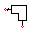
\includegraphics[width=12cm]{mscorner}
\end{center}
\caption{microstrip corner (left), mitered corner (middle) and equivalent circuit (right)}
\label{fig:MScorner}
\end{figure}
\FloatBarrier

The Z-parameters for the given equivalent small signal circuit can be
written as stated in eq. \eqref{eq:MScornerZ} and are easy to convert
to scattering parameters.
\begin{equation}
Z =
\begin{bmatrix}
j\omega L + \dfrac{1}{j\omega C} & \dfrac{1}{j\omega C}\\
\dfrac{1}{j\omega C} & j\omega L + \dfrac{1}{j\omega C}\\
\end{bmatrix}
\label{eq:MScornerZ}
\end{equation}

\section{Parallel coupled microstrip lines}
%\addcontentsline{toc}{section}{Parallel coupled microstrip lines}

\begin{figure}[ht]
\begin{center}
\includegraphics[width=12cm]{mscoupledphys}
\end{center}
\caption{parallel coupled microstrip lines}
\label{fig:McoupledPhys}
\end{figure}
\FloatBarrier

\subsection{Characteristic impedance and effective dielectric constant}
%\addcontentsline{toc}{subsection}{Characteristic impedance and effective dielectric constant}

Parallel coupled microstrip lines are defined by the characteristic
impedance and the effective permittivity of the even and the odd mode.

\subsubsection{Kirschning and Jansen}
%\addcontentsline{toc}{subsubsection}{Kirschning and Jansen}

These quantities can very precisely be modeled by the following
equations \cite{Kirschning2}, \cite{Kirschning6}.

\addvspace{12pt}

Beforehand some normalised quantities (with microstrip line width $W$,
spacing $s$ between the lines and substrate height $h$) are
introduced:
\begin{equation}
u = \dfrac{W}{h} \quad,\quad g = \dfrac{s}{h} \quad,\quad
f_n = \dfrac{f}{\giga\hertz}\cdot\dfrac{h}{\milli\meter} = \dfrac{f}{\mega\hertz}\cdot h
\end{equation}

The applicability of the described model is
\begin{equation}
0.1\le u\le 10 \qquad,\qquad 0.1\le g\le 10 \qquad,\qquad 1\le \varepsilon_r\le 18
\end{equation}
The accuracies of the formulas holds for these ranges.

\addvspace{12pt}

Static effective permittivity of even mode:
\begin{equation}
\varepsilon_{eff,e}(0) = 0.5\cdot (\varepsilon_r+1) + 0.5\cdot (\varepsilon_r-1)\cdot
      \left( 1+\dfrac{10}{v} \right) ^{-a_e\left(v\right)\cdot b_e\left(\varepsilon_r\right)}
\end{equation}

with
\begin{align}
v &= u\cdot\frac{20+g^2}{10+g^2} + g\cdot\exp{\left(-g\right)}\\
a_e\left(v\right) &= 1 + \frac{1}{49}\cdot\ln\left( \frac{v^4 + \left( v/52 \right)^2}{v^4 + 0.432} \right)
    + \frac{1}{18.7}\cdot\ln\left( 1 + \left( \dfrac{v}{18.1} \right)^3 \right)\\
b_e\left(\varepsilon_r\right) &= 0.564\cdot\left( \frac{\varepsilon_r-0.9}{\varepsilon_r+3} \right)^{0.053}
\end{align}

Static effective permittivity of odd mode:
\begin{equation}
\varepsilon_{eff,o}(0) = \left(0.5\cdot \left(\varepsilon_r+1\right) + a_o\left(u,\varepsilon_r\right) - \varepsilon_{eff}(0) \right) \cdot
      \exp{\left(-c_o\cdot g^{d_o}\right)} + \varepsilon_{eff}(0)
\end{equation}

with
\begin{align}
a_o\left(u,\varepsilon_r\right) &= 0.7287\cdot\left( \varepsilon_{eff}(0) - 0.5\cdot \left( \varepsilon_r + 1\right) \right) \cdot
      \left(1-\exp{\left(-0.179\cdot u\right)}\right)\\
b_o\left(\varepsilon_r\right) &= 0.747\cdot\dfrac{\varepsilon_r}{0.15+\varepsilon_r}\\
c_o &= b_o(\varepsilon_r) - \left(b_o\left(\varepsilon_r\right)-0.207\right)\cdot\exp{\left(-0.414\cdot u\right)}\\
d_o &= 0.593+0.694\cdot\exp{\left(-0.562\cdot u\right)}
\end{align}

whence $\varepsilon_{eff}(0)$ refers to the zero-thickness single
microstrip line of width $W$ according to \cite{Hammerstad} (see also
eq. \eqref{eq:HandJErEff}).

\addvspace{12pt}

The dispersion formulae for the odd and even mode write as follows.
\begin{equation}
\varepsilon_{eff,e,o}\left(f_n\right) = \varepsilon_r - \dfrac{\varepsilon_r - \varepsilon_{eff,e,o}(0)}{1+F_{e,o}\left(f_n\right)}
\end{equation}

The frequency dependence for the even mode is
\begin{equation}
F_e\left(f_n\right) = P_1\cdot P_2\cdot \left(\left(P_3\cdot P_4 + 0.1844\cdot P_7\right)\cdot f_n\right)^{1.5763}
\end{equation}

with
\begin{align}
P_1 &= 0.27488 + \left( 0.6315 + \dfrac{0.525}{(1+0.0157\cdot f_n)^{20}} \right) \cdot u
     -0.065683\cdot\exp{\left(-8.7513\cdot u\right)}\\
P_2 &= 0.33622\cdot \left(1-\exp{\left(-0.03442\cdot\varepsilon_r\right)}\right)\\
P_3 &= 0.0363\cdot\exp{\left(-4.6\cdot u\right)}\cdot\left( 1-\exp\left(
    -\left( f_n / 38.7\right) ^{4.97} \right) \right)\\
P_4 &= 1 + 2.751\cdot\left( 1-\exp\left( -\left( \varepsilon_r/15.916\right) ^8 \right) \right)\\
P_5 &= 0.334\cdot\exp\left( -3.3\cdot\left( \varepsilon_r/15\right) ^3 \right) + 0.746\\
P_6 &= P_5\cdot\exp\left( -\left( f_n/18\right) ^{0.368} \right)\\
P_7 &= 1 + 4.069\cdot P_6 \cdot g^{0.479}\cdot\exp\left(-1.347\cdot g^{0.595} - 0.17\cdot g^{2.5} \right)
\end{align}

The frequency dependence for the odd mode is
\begin{equation}
F_o\left(f_n\right) = P_1\cdot P_2\cdot \left(\left(P_3\cdot P_4 + 0.1844\right)\cdot f_n\cdot P_{15}\right)^{1.5763}
\end{equation}

with
\begin{align}
P_8 &= 0.7168\cdot \left(1 + \frac{1.076}{1+0.0576\cdot \left(\varepsilon_r-1\right)} \right)\\
P_9 &= P_8 - 0.7913\cdot\left( 1-\exp\left( -\left( f_n/20\right) ^{1.424} \right) \right)
     \cdot\arctan\left( 2.481\cdot\left( \varepsilon_r/8\right) ^{0.946} \right)\\
P_{10} &= 0.242\cdot \left(\varepsilon_r-1\right)^{0.55}\\
P_{11} &= 0.6366\cdot \left(\exp\left(-0.3401\cdot f_n\right)-1\right) \cdot
      \arctan\left(1.263\cdot\left( u/3 \right) ^{1.629} \right)\\
P_{12} &= P_9 + \dfrac{1-P_9}{1+1.183\cdot u^{1.376}}\\
P_{13} &= 1.695\cdot \dfrac{P_{10}}{0.414+1.605\cdot P_{10}}\\
P_{14} &= 0.8928 + 0.1072\cdot \left( 1-\exp\left(-0.42\cdot\left(
        f_n/20 \right) ^{3.215} \right)\right)\\
P_{15} &= \left| 1 - 0.8928\cdot \left(1+P_{11}\right) \cdot \exp\left(-P_{13}\cdot g^{1.092}\right)\cdot
         P_{12}/P_{14} \right|
\end{align}

Up to $f_n=25$ the maximum error of these equations is 1.4\%.

\addvspace{12pt}

The static characteristic impedance for the even mode writes as follows.
\begin{equation}
Z_{L,e}(0) = \sqrt{\dfrac{\varepsilon_{eff}(0)}{\varepsilon_{eff,e}(0)}} \cdot
             \dfrac{Z_L(0)}{1 - \dfrac{Z_L(0)}{377\ohm} \cdot \sqrt{\varepsilon_{eff}(0)} \cdot Q_4}
\end{equation}

with
\begin{align}
Q_1 &= 0.8695\cdot u^{0.194}\\
Q_2 &= 1 + 0.7519\cdot g + 0.189\cdot g^{2.31}\\
Q_3 &= 0.1975 + \left( 16.6 + \left( 8.4/g \right) ^6 \right) ^{-0.387}
     + \dfrac{1}{241} \cdot \ln\left( \dfrac{g^{10}}{1+\left( g/3.4\right) ^{10}} \right)\\
Q_4 &= \frac{Q_1}{Q_2}\cdot \frac{2}{ \exp\left(-g\right)\cdot u^{Q_3} + (2-\exp\left(-g\right))\cdot u^{-Q_3} }
\end{align}

with $Z_L(0)$ and $\varepsilon_{eff}(0)$ being again quantities for a
zero-thickness single microstrip line of width $W$ according to
\cite{Hammerstad} (see also eq. \eqref{eq:HandJErEff} and
\eqref{eq:HandJZL0Er}).

\addvspace{12pt}

The static characteristic impedance for the odd mode writes as follows.
\begin{equation}
Z_{L,o}(0) = \sqrt{\dfrac{\varepsilon_{eff}(0)}{\varepsilon_{eff,o}(0)}} \cdot
             \dfrac{Z_L(0)}{1 - \dfrac{Z_L(0)}{377\Omega} \cdot \sqrt{\varepsilon_{eff}(0)} \cdot Q_{10}}
\end{equation}

with
\begin{align}
Q_5 &= 1.794 +1.14\cdot\ln\left( 1 + \frac{0.638}{g+0.517\cdot g^{2.43}} \right)\\
Q_6 &= 0.2305 + \frac{1}{281.3}\cdot \ln\left( \frac{g^{10}}{1+\left( g/5.8\right) ^{10}} \right)
     + \frac{1}{5.1}\cdot \ln\left(1+0.598\cdot g^{1.154}\right)\\
Q_7 &= \frac{10+190\cdot g^2}{1+82.3\cdot g^3}\\
Q_8 &= \exp\left( -6.5 - 0.95\cdot\ln\left(g\right) - \left(g/0.15\right)^5 \right)\\
Q_9 &= \ln\left(Q_7\right)\cdot \left( Q_8 + 1/16.5 \right)\\
Q_{10} &= \frac{Q_2\cdot Q_4 - Q_5\cdot\exp\left( \ln\left(u\right)\cdot Q_6\cdot u^{-Q_9} \right)}{Q_2}
       = Q_4 - \frac{Q_5}{Q_2}\cdot u^{Q_6\cdot u^{-Q_9}}
\end{align}

The accuracy of the static impedances is better than 0.6\%.

\addvspace{12pt}

Dispersion of the characteristic impedance for the even mode can be
modeled by the following equations.
\begin{equation}
Z_{L,e}(f_n) = Z_{L,e}(0)\cdot \left( \dfrac{0.9408\cdot (\varepsilon_{eff}(f_n))^{C_e} - 0.9603}
                        {\left(0.9408-d_e\right)\cdot \left(\varepsilon_{eff}(0)\right)^{C_e} - 0.9603} \right) ^{Q_0}
\end{equation}

with
\begin{equation}
\begin{split}
C_e = 1 + 1.275\cdot \left( 1-\exp\left( -0.004625\cdot p_e\cdot \varepsilon_r^{1.674}\cdot
      \left( f_n/18.365 \right) ^{2.745} \right) \right)\\
      - Q_{12}+Q_{16}-Q_{17}+Q_{18}+Q_{20}
\end{split}
\end{equation}
\begin{align}
d_e &= 5.086\cdot q_e\cdot\dfrac{r_e}{0.3838+0.386\cdot q_e}\cdot
      \dfrac{\exp\left(-22.2\cdot u^{1.92}\right)}{1+1.2992\cdot r_e}\cdot
      \dfrac{(\varepsilon_r-1)^6}{1 + 10\cdot (\varepsilon_r-1)^6}\\
p_e &= 4.766\cdot \exp \left(-3.228\cdot u^{0.641}\right)\\
q_e &= 0.016 + \left(0.0514\cdot \varepsilon_r\cdot Q_{21}\right)^{4.524}\\
r_e &= \left( f_n/28.843 \right) ^{12}
\end{align}

and
\begin{align}
Q_{11} &= 0.893\cdot \left( 1 - \frac{0.3}{1+0.7\cdot\left(\varepsilon_r-1\right)} \right)\\
Q_{12} &= 2.121\cdot \frac{\left( f_n/20\right) ^{4.91}}
                         {1+Q_{11}\cdot\left( f_n/20\right) ^{4.91}}
	      \cdot \exp\left(-2.87\cdot g\right)\cdot g^{0.902}\\
Q_{13} &= 1 + 0.038\cdot \left( \varepsilon_r/8 \right) ^{5.1}\\
Q_{14} &= 1 + 1.203\cdot \dfrac{ \left( \varepsilon_r/15 \right) ^4}
                             {1 + \cdot \left( \varepsilon_r/15 \right) ^4}\\
Q_{15} &= \dfrac{ 1.887\cdot \exp\left(-1.5\cdot g^{0.84}\right)\cdot g^{Q_{14}} }
              { 1 + 0.41\cdot \left( f_n/15 \right) ^3 \cdot
	        \dfrac{u^{2/Q_{13}}}{0.125 + u^{1.626/Q_{13}}}}\\
Q_{16} &= Q_{15}\cdot \left( 1 + \frac{9}{1+0.403\cdot \left(\varepsilon_r-1\right)^2} \right)\\
Q_{17} &= 0.394\cdot \left( 1-\exp\left( -1.47\cdot\left( u/7 \right) ^{0.672} \right) \right)
        \cdot \left( 1-\exp\left( -4.25\left( f_n/20 \right) ^{1.87} \right) \right)\\
Q_{18} &= 0.61\cdot\frac{1-\exp\left( -2.13\cdot\left( u/8 \right) ^{1.593} \right)}
                  {1+6.544\cdot g^{4.17}}\\
Q_{19} &= \frac{ 0.21\cdot g^4 }{\left(1+0.18\cdot g^{4.9}\right)\cdot \left(1+0.1\cdot u^2\right) \cdot
                \left( 1+\left( f_n/24 \right) ^3 \right)}\\
Q_{20} &= Q_{19}\cdot \left( 0.09 + \frac{1}{1+0.1\cdot \left(\varepsilon_r-1\right)^{2.7}} \right)\\
Q_{21} &= \left| 1-42.54\cdot g^{0.133}\cdot \exp\left(-0.812\cdot g\right)
                   \cdot\frac{u^{2.5}}{1+0.033\cdot u^{2.5}} \right|
\end{align}

With $\varepsilon_{eff}(f_n)$ being the single microstrip effective
dielectric constant according to \cite{Kirschning3} (see eq.
\eqref{eq:KandJErEff_disp}) and $Q_0$ single microstrip impedance
dispersion according to \cite{Kirschning1} (there denoted as $R_{17}$,
see eq. \eqref{eq:KirschningR17}).

\addvspace{12pt}

Dispersion of the characteristic impedance for the odd mode can be
modeled by the following equations.
\begin{equation}
Z_{L,o}(f_n) = Z_L(f_n) + \dfrac{ Z_{L,o}(0)\cdot
               \left( \dfrac{\varepsilon_{eff,o}(f_n)}{\varepsilon_{eff,o}(0)} \right) ^{Q_{22}}
	     - Z_L(f_n)\cdot Q_{23} }{ 1+Q_{24}+\left(0.46\cdot g\right)^{2.2} \cdot Q_{25} }
\end{equation}

with
\begin{align}
Q_{22} &= 0.925\cdot \frac{ \left( f_n/Q_{26} \right) ^{1.536} }
                         { 1+0.3\cdot \left( f_n/30 \right)^{1.536} }\\
Q_{23} &= 1+ \frac{ 0.005\cdot f_n\cdot Q_{27} }
                 { \left( 1+0.812\cdot\left( f_n/15 \right) ^{1.9} \right) \cdot
		   \left(1 + 0.025\cdot u^2\right) }\\
Q_{24} &= \frac{2.506\cdot Q_{28}\cdot u^{0.894}}{3.575+u^{0.894}} \cdot
         \left( \frac{ (1+1.3\cdot u)\cdot f_n}{99.25} \right)^{4.29}\\
Q_{25} &= \frac{0.3\cdot f_n^2}{10+f_n^2}\cdot
         \left( 1+ \frac{2.333\cdot \left(\varepsilon_r-1\right)^2}{5+\left(\varepsilon_r-1\right)^2} \right)\\
Q_{26} &= 30 - \frac{ 22.2\cdot \left( \dfrac{\varepsilon_r-1}{13} \right)^{12} }
                   { 1+ 3\cdot \left( \dfrac{\varepsilon_r-1}{13} \right)^{12} } - Q_{29}\\
Q_{27} &= 0.4\cdot g^{0.84}\cdot \left( 1+
         \frac{2.5\cdot \left(\varepsilon_r-1\right)^{1.5}}{5+\left(\varepsilon_r-1\right)^{1.5}} \right)\\
Q_{28} &= 0.149\cdot \frac{\left(\varepsilon_r-1\right)^3}{94.5+0.038\cdot \left(\varepsilon_r-1\right)^3}\\
Q_{29} &= \frac{15.16}{1+0.196\cdot \left(\varepsilon_r-1\right)^2}
\end{align}

with $Z_L(f_n)$ being the frequency-dependent power-current
characteristic impedance formulation of a single microstrip with width
$W$ according to \cite{Kirschning1} (see
eq. \eqref{eq:KirschningZLdisp}).  Up to $f_n=20$, the numerical error
of $Z_{L,o}(f_n)$ and $Z_{L,e}(f_n)$ is less than 2.5\%.

\subsubsection{Hammerstad and Jensen}
%\addcontentsline{toc}{subsubsection}{Hammerstad and Jensen}

The equations given by E. Hammerstad and {\O}. Jensen
\cite{Hammerstad} represent the first generally valid model of coupled
microstrips with an acceptable accuracy.  The model equations have
been validated in the range $0.1 \le u \le 10$ and $g \ge 0.01$, a
range which should cover that used in practice.

\addvspace{12pt}

The homogeneous mode impedances are
\begin{equation}
\label{eq:HandJZLeo}
Z_{L,e,o}\left(u, g\right) = \dfrac{Z_{L}(u)}{1 - Z_{L}(u)\cdot \Phi_{e,o}\left(u,g\right) / Z_{F0}}
\end{equation}

The effective dielectric constants are
\begin{equation}
\varepsilon_{eff,e,o}\left(u,g,\varepsilon_r\right) = \dfrac{\varepsilon_r+1}{2} + \dfrac{\varepsilon_r-1}{2}\cdot F_{e,o}\left(u,g,\varepsilon_r\right)
\end{equation}

with
\begin{align}
F_{e}\left(u,g,\varepsilon_r\right) &= \left(1+\dfrac{10}{\mu\left(u,g\right)}\right)^{-a(\mu)\cdot b\left(\varepsilon_r\right)}\\
F_{o}\left(u,g,\varepsilon_r\right) &= f_o\left(u,g,\varepsilon_r\right)\cdot \left(1+\dfrac{10}{u}\right)^{-a\left(u\right)\cdot b\left(\varepsilon_r\right)}
\end{align}

whence $a(u)$ and $b\left(\varepsilon_r\right)$ denote
eqs. \eqref{eq:HandJa} and \eqref{eq:HandJb} of the single microstrip
line.  The characteristic impedance of the single microstrip line
$Z_L\left(u\right)$ also defined in \cite{Hammerstad} is given by
eq. \eqref{eq:HandJZL0Er}.  The modifying equations for the even mode
are as follows
\begin{align}
\Phi_e\left(u,g\right) &= \dfrac{\varphi(u)}{\Psi(g)\cdot \left(\alpha(g)\cdot u^{m(g)} +\left(1-\alpha(g)\right)\cdot u^{-m(g)}\right)}\\
% TODO: is this ... Psi * (Alpha ... or ... Psi / (Alpha ... ?
\varphi(u) &= 0.8645\cdot u^{0.172}\\
\Psi(g) &= 1 + \dfrac{g}{1.45} + \dfrac{g^{2.09}}{3.95}\\
\alpha(g) &= 0.5\cdot e^{-g}\\
m(g) &= 0.2175+\left(4.113+\left(20.36/g\right)^6\right)^{-0.251} +\dfrac{1}{323}\cdot\ln{\left(\dfrac{g^{10}}{1+\left(g/13.8\right)^{10}}\right)}
\end{align}

The modifying equations for the odd mode are as follows
\begin{align}
\Phi_o\left(u,g\right) &= \Phi_e\left(u,g\right)-\dfrac{\theta(g)}{\Psi(g)}\cdot \exp{\left(\beta(g)\cdot u^{-n(g)}\cdot\ln{u}\right)}\\
\theta(g) &= 1.729+1.175\cdot\ln{\left(1+\dfrac{0.627}{g+0.327\cdot g^{2.17}}\right)}\\
\beta(g) &= 0.2306+\dfrac{1}{301.8}\cdot\ln{\left(\dfrac{g^{10}}{1+\left(g/3.73\right)^{10}}\right)} +\dfrac{1}{5.3}\cdot\ln{\left(1+0.646\cdot g^{1.175}\right)}\\
n(g) &= \left(\dfrac{1}{17.7} + \exp{\left(-6.424 - 0.76\cdot \ln{g} - \left(g/0.23\right)^5\right)}\right)\cdot \ln{\left(\dfrac{10 + 68.3\cdot g^2}{1+32.5\cdot g^{3.093}}\right)}
\end{align}

Furthermore
\begin{align}
\mu\left(u,g\right) &= g\cdot e^{-g}+ u\cdot \dfrac{20+g^2}{10+g^2}\\
f_o\left(u,g,\varepsilon_r\right) &= f_{o1}\left(g,\varepsilon_r\right)\cdot \exp{\left(p(g)\cdot \ln{u} + q(g)\cdot \sin{\left(\pi\cdot\log{u}\right)}\right)}\\
p(g) &= \dfrac{\exp{\left(-0.745\cdot g^{0.295}\right)}}{\cosh{\left(g^{0.68}\right)}}\\
q(g) &= \exp{\left(-1.366-g\right)}\\
f_{o1}\left(g,\varepsilon_r\right) &= 1 - \exp{\left(-0.179\cdot g^{0.15} - \dfrac{0.328\cdot g^{r\left(g,\varepsilon_r\right)}}{\ln{\left(e + \left(g/7\right)^{2.8}\right)}}\right)}\\
r\left(g,\varepsilon_r\right) &= 1+0.15\cdot\left(1 - \dfrac{\exp{\left(1-\left(\varepsilon_r - 1\right)^2/8.2\right)}}{1+g^{-6}}\right)
\end{align}

The quasi-static characteristic impedance $Z_L(u)$ of a zero-thickness
single microstrip line denoted in eq. \eqref{eq:HandJZLeo} can either
be calculated using the below equations with $\varepsilon_{r_{eff}}$
being the quasi-static effective dielectric constant defined by
eq. \eqref{eq:HandJErEff} or using eqs. \eqref{eq:HandJZL0Er} and
\eqref{eq:HandJErEff}.
\begin{align}
Z_{L1}(u) &= \dfrac{Z_{F0}}{u + 1.98\cdot u^{0.172}}\\
Z_{L}(u) &= \dfrac{Z_{L1}(u)}{\sqrt{\varepsilon_{r_{eff}}}}
\end{align}

The errors in the even and odd mode impedances $Z_{L,e}$ and $Z_{L,e}$
were found to be less than 0.8\% and less than 0.3\% for the
wavelengths.

\addvspace{12pt}

The model does not include the effect of non-zero strip thickness or
asymmetry.  Dispersion is also not included.  W. J. Getsinger
\cite{Getsinger4} has proposed modifications to his single strip
dispersion model, but unfortunately it is easily shown that the
results are asymptotically wrong for extreme values of gap width.

\addvspace{12pt}

In fact he correctly assumes that in the even mode the two strips are
at the same potential, and the total current is twice that on a single
strip, and dispersion for even-mode propagation is computed by
substituting $Z_{L,e}/2$ for $Z_L$ in eqs. \eqref{eq:GetFp} and
\eqref{eq:GetG}.  In the odd mode the two strips are at opposite
potentials, and the voltage between strips is twice that of a single
strip to ground.  Thus the total mode impedance is twice that of a
single strip, and the dispersion for odd-mode propagation is computed
substituting $2Z_{L,o}$ for $Z_L$ in eqs. \eqref{eq:GetFp} and
\eqref{eq:GetG}.
\begin{equation}
\varepsilon_{r,e,o}\left(f\right) = \varepsilon_{r} - \frac{\varepsilon_{r} - \varepsilon_{r_{eff,e,o}}}{1 + G\cdot \left(\dfrac{f}{f_{p}}\right)^{2}}
\end{equation}

with
\begin{align}
f_{p} &=
\begin{cases}
\begin{array}{ll}
\dfrac{Z_{L,e}}{4\mu_{0} h} & \textrm{ even mode }\\&\\
\dfrac{Z_{L,o}}{\mu_{0} h}  & \textrm{ odd mode }\\
\end{array}
\end{cases}\\
G &=
\begin{cases}
\begin{array}{ll}
0.6 + Z_{L,e}\cdot 0.0045 & \textrm{ even mode }\\&\\
0.6 + Z_{L,o}\cdot 0.018 & \textrm{ odd mode }\\
\end{array}
\end{cases}
\end{align}

\subsection{Transmission losses}
%\addcontentsline{toc}{subsection}{Transmission losses}

The loss equations given by E. Hammerstad and {\O}. Jensen
\cite{Hammerstad} for the single microstrip line are also valid for
coupled microstrips, provided that the dielectric filling factor,
homogeneous impedance, and current distribution factor of the actual
mode are used.  The following approximation gives good results for odd
and even current distribution factors (modification of
eq. \eqref{eq:HandJKi}).

\begin{equation}
K_e = K_o = \exp{\left(-1.2\cdot\left(\dfrac{Z_{L,e} + Z_{L,o}}{2\cdot Z_{F0}}\right)^{0.7}\right)}
\end{equation}

\subsection{S-parameters of parallel coupled microstrip lines}
%\addcontentsline{toc}{subsection}{S-parameters of parallel coupled microstrip lines}

After endless equations formulating the effective dielectric constant
and the characte\-ris\-tic impe\-dance of the even and odd mode, the
S-parameters (according to the port numbering in
fig. \ref{fig:mscoupled}) can now be defined \cite{Edwards}.

\addvspace{12pt}

reflection coefficients
\begin{equation}
S_{11} = S_{22} = S_{33} = S_{44} = X_e + X_o
\end{equation}
through paths
\begin{equation}
S_{12} = S_{21} = S_{34} = S_{43} = Y_e + Y_o
\end{equation}
coupled paths
\begin{equation}
S_{14} = S_{41} = S_{23} = S_{32} = X_e - X_o
\end{equation}
isolated paths
\begin{equation}
S_{13} = S_{31} = S_{24} = S_{42} = Y_e - Y_o
\end{equation}

with the denominator
\begin{equation}
D_{e,o} = 2\cdot Z_{L,e,o}\cdot Z_0\cdot \cosh(\gamma_{e,o}\cdot l)
         + \left(Z_{L,e,o}^2 + Z_0^2\right)\cdot \sinh\left(\gamma_{e,o}\cdot l\right)
\end{equation}

and
\begin{align}
X_{e,o} &= \frac{\left(Z_{L,e,o}^2 - Z_0^2\right)\cdot \sinh\left(\gamma_{e,o}\cdot l\right)}{2\cdot D_{e,o}}\\
Y_{e,o} &= \frac{Z_{L,e,o}\cdot Z_0}{D_{e,o}}
\end{align}

\begin{figure}[ht]
\begin{center}
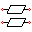
\includegraphics[width=0.5\linewidth]{mscoupled}
\end{center}
\caption{coupled microstrip line}
\label{fig:mscoupled}
\end{figure}
\FloatBarrier

\section{Microstrip open}
%\addcontentsline{toc}{section}{Microstrip open}

A microstrip open end can be modeled by a longer effective microstrip
line length $\Delta l$ as described by M. Kirschning, R.H. Jansen and
N.H.L. Koster \cite{Kirschning7}.
\begin{equation}
\frac{\Delta l}{h} = \frac{Q_1\cdot Q_3\cdot Q_5}{Q_4}
\end{equation}

with
\begin{align}
Q_1 &= 0.434907\cdot \dfrac{\varepsilon_{r,eff}^{0.81}+0.26}{\varepsilon_{r,eff}^{0.81}-0.189}\cdot
      \dfrac{\left( W/h \right)^{0.8544} + 0.236}{\left( W/h \right)^{0.8544} + 0.87}\\
Q_2 &= 1 + \dfrac{\left( W/h \right) ^{0.371}}{2.358\cdot \varepsilon_r + 1}\\
Q_3 &= 1 + \dfrac{0.5274}{\varepsilon_{r,eff}^{0.9236}} \cdot
      \arctan\left( 0.084\cdot\left( W/h \right) ^{\tfrac{1.9413}{Q_2}} \right)\\
Q_4 &= 1 + 0.0377\cdot \left( 6-5\cdot\exp{\left(0.036\cdot\left(1-\varepsilon_r\right)\right)} \right)\cdot
      \arctan\left( 0.067\cdot\left(W/h\right)^{1.456} \right)\\
Q_5 &= 1 - 0.218\cdot \exp{\left( -7.5\cdot W/h \right)}
\end{align}

The numerical error is less than $2.5$\% for $0.01\le W/h \le 100$ and
$1\le\varepsilon_r\le 50$.

\addvspace{12pt}

Another microstrip open end model was published by E. Hammerstad
\cite{Hammerstad2}:
\begin{equation}
\dfrac{\Delta l}{h} = 0.102\cdot \dfrac{W/h+0.106}{W/h+0.264} \cdot
    \left( 1.166 + \dfrac{\varepsilon_r+1}{\varepsilon_r}\cdot \left(0.9+\ln{\left(W/h+2.475\right)} \right) \right)
\end{equation}

Here the numerical error is less than $1.7$\% for $W/h < 20$.

\addvspace{12pt}

In order to simplify calculations, the equivalent additional line
length $\Delta l$ can be transformed into an equivalent open end
capacitance $C_{end}$:
\begin{equation}
\label{eq:Cend}
C_{end} = C'\cdot \Delta l = \dfrac{\sqrt{\varepsilon_{r,eff}}}{c_0\cdot Z_L} \Delta l
\end{equation}

With $C'$ being the capacitance per length and $c_0$ = 299 792 458 m/s
being the vacuum light velocity.

\section{Microstrip gap}
%\addcontentsline{toc}{section}{Microstrip gap}

A symmetrical microstrip gap can be modeled by two open ends with a
capacitive series coupling between the two ends.  The physical layout
is shown in fig. \ref{fig:MSgaPhys}.

\begin{figure}[ht]
\begin{center}
\includegraphics[width=8cm]{msgapphys}
\end{center}
\caption{symmetrical microstrip gap layout}
\label{fig:MSgaPhys}
\end{figure}
\FloatBarrier

The equivalent $\pi$-network of a microstrip gap is shown in figure
\ref{fig:MSgap}.  The values of the components are according to
\cite{Kirschning8} and \cite{Kirschning4}.
\begin{equation}
C_S \textrm{ [pF] } = 500\cdot h\cdot\exp\left( -1.86\cdot\dfrac{s}{h} \right)\cdot Q_1\cdot
       \left( 1 + 4.19\left( 1 - \exp\left( -0.785\cdot\sqrt{\dfrac{h}{W_1}}\cdot
       \dfrac{W_2}{W_1} \right) \right) \right)
\end{equation}
\begin{align}
C_{P1} &= C_1\cdot \dfrac{Q_2+Q_3}{Q_2+1}\\
C_{P2} &= C_2\cdot \dfrac{Q_2+Q_4}{Q_2+1}
\end{align}

with
\begin{align}
Q_1 &= 0.04598\cdot \left( 0.03 + \left(\frac{W_1}{h}\right)^{Q_5} \right)\cdot
      (0.272 + 0.07\cdot\varepsilon_r)\\
Q_2 &= 0.107\cdot\left( \frac{W_1}{h}+9 \right) \cdot \left( \dfrac{s}{h} \right)^{3.23}
    + 2.09 \cdot \left( \dfrac{s}{h} \right)^{1.05}\cdot
    \frac{1.5+0.3\cdot W_1/h}{1+0.6\cdot W_1/h}\\
Q_3 &= \exp\left( -0.5978\cdot \left( \frac{W_2}{W_1} \right)^{1.35} \right) - 0.55\\
Q_4 &= \exp\left( -0.5978\cdot \left( \frac{W_1}{W_2} \right)^{1.35} \right) - 0.55\\
Q_5 &= \frac{1.23}{1 + 0.12\cdot \left( W_2 / W_1 - 1 \right)^{0.9}}
\end{align}

with $C_1$ and $C_2$ being the open end capacitances of a microstrip
line (see eq. \eqref{eq:Cend}).  The numerical error of the
capacitive admittances is less than $0.1$mS for
\begin{equation*}
\begin{split}
0.1\le W_1/h \le 3 \\
0.1\le W_2/h \le 3 \\
1\le W_2/W_1 \le 3 \\
6\le \varepsilon_r \le 13 \\
0.2\le s/h \le \infty \\
0.2\text{GHz} \le f \le 18\text{GHz}
\end{split}
\end{equation*}

\begin{figure}[ht]
\begin{center}
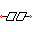
\includegraphics[width=12cm]{msgap}
\end{center}
\caption{microstrip gap and its equivalent circuit}
\label{fig:MSgap}
\end{figure}
\FloatBarrier

The Y-parameters for the given equivalent small signal circuit can be
written as stated in eq. \eqref{eq:MSgapY} and are easy to convert to
scattering parameters.
\begin{equation}
Y =
\begin{bmatrix}
j\omega\cdot \left(C_{P1} + C_S\right) & -j\omega C_S\\
-j\omega C_S & j\omega\cdot \left(C_{P2} + C_S\right)\\
\end{bmatrix}
\label{eq:MSgapY}
\end{equation}

\section{Microstrip impedance step}
%\addcontentsline{toc}{section}{Microstrip impedance step}

The equivalent circuit of a microstrip impedance step is the same as
for the microstrip corner (figure \ref{fig:MScorner}).  The values are
according to \cite{Gupta}:
\begin{equation}
C_S \textrm{ [pF] } = \sqrt{W_1\cdot W_2}\cdot\left( (10.1\cdot\log{\varepsilon_r} + 2.33)\cdot
     \dfrac{W_1}{W_2} - 12.6\cdot\log{\varepsilon_r} - 3.17 \right)
\end{equation}

for $\varepsilon_r\le 10$ and $1.5\le W_1/W_2\le 3.5$ the error is
$<10$\%.
\begin{equation}
L_1 = \frac{L_{W1}}{L_{W1}+L_{W2}}\cdot L_S
\end{equation}
\begin{equation}
L_2 = \frac{L_{W2}}{L_{W1}+L_{W2}}\cdot L_S
\end{equation}

with
\begin{equation}
L_{W1,2} = \dfrac{Z_{L,1,2}\cdot\sqrt{\varepsilon_{r,eff,1,2}}}{c_0}
\end{equation}
\begin{equation}
\frac{L_S}{h} \textrm{ [nH/m] } = 40.5\cdot\left( \dfrac{W_1}{W_2}-1 \right)
      - 75\cdot\log{\dfrac{W_1}{W_2}} + 0.2\cdot \left( \dfrac{W_1}{W_2}-1 \right)^2
\end{equation}
With $c_0$ = 299 792 458 m/s being the vacuum light velocity.  The
error is less than 5\% for $W_1/W_2\le 5$ and $W_2/h = 1$.

\section{Microstrip tee junction}
%\addcontentsline{toc}{section}{Microstrip tee junction}

\section{Microstrip cross}
%\addcontentsline{toc}{section}{Microstrip cross}

